\documentclass[10pt,conference]{IEEEtran}
%\documentclass[a4paper,12pt]{article}
%\usepackage{algpseudocode}
\usepackage{cite,latexsym,times,epsf,amsmath,amssymb,amsfonts,graphicx}
\usepackage{epstopdf}
\usepackage{graphicx}
\usepackage{subfigure}
\usepackage{multirow}
\usepackage{algorithmic}
\usepackage{algorithm}
\usepackage{amsmath}
\usepackage{verbatim}
\usepackage{booktabs}



\renewcommand{\algorithmicrequire}{\textbf{Input:}}
\renewcommand{\algorithmicensure}{\textbf{Output:}}
\renewcommand{\baselinestretch}{0.95}
%\renewcommand{\algorithmicforall}{\textbf{Foreach}}
%\renewcommand{\algorithmicendfor}{\textbf{}}


\begin{document}
\title{Beamforming Mesh Deployment}
\author{ TBA\\ 
Department of Electrical Engineering, Southern Methodist University, Dallas, TX \\
%\{camp\}@smu.edu  \\
}


%\documentclass[10pt]{article}

%\usepackage{xkvltxp}


\maketitle
\begin{abstract}

\end{abstract}

%\section{Introduction}
\label{sec:introduction}

% Dployment constraints: QOS, capacity; coverage; resource constraint
% Beamforming
% Problem: beamforming in differet QoS environments
% Beamforming benefit in network deployment
% Issues
% Paper organization


% Background multiband, propagation diversity
The FCC has approved the use of broadband services in the white spaces of 
UHF TV bands, which were formerly exclusively licensed to television broadcasters.
These white space bands are now available for unlicensed public use, enabling the
deployment of wireless access networks across a broad range of scenarios from 
sparse rural areas (one of the key applications identified by the FCC) to dense urban 
areas~\cite{carlson}. The white space bands operate in available channels from 
54-806 MHz, having a far greater propagation range than WiFi bands for similar
transmission power~\cite{balanis2012antenna}. 

Specific to rural areas, the lack of user density and corresponding traffic
demand per unit area as compared to dense urban areas allows greater levels of
spatial aggregation to reduce the total number of required access points, lowering
network deployment costs. In densely populated urban areas, the greater concentration
of users and higher levels of traffic demand can be served by maximizing the spatial
reuse. While many works have worked to address multihop wireless network deployment
in terms of maximizing served user demand and/or minimizing network costs,
the unique deployment heterogeneous access points of white space bands and 
WiFi bands have either not been studied~\cite{si2010overview}. 
Specifically, previous work has investigated wireless network deployment in terms of 
multiradio network, power control, gateway placement, channel assignment, 
and routing~\cite{kodialam2005characterizing,he2008optimizing,marina2010topology}.
However, each of these works focus on the deployment in WiFi bands without
considering the white space bands. The white space band could extend the capacity 
degree and the coverage degree of an access point simultaneous. 

In WiFi and white space heterogeneous wireless network, the service area degree of 
an access point depends on the capacity of radios, the propagation range and the 
demands of the serving area. The scant frequencies of radios, the propagation distinctive
and the demands diversity of population distribution bring the variation of an access point
service area. These issues are substantial to designing an optimal network deployment 
and provide potential commercial wireless services to clients in any location.

Thus, the new opportunities created by white spaces motivate the following 
questions for wireless Internet carriers, which have yet to be addressed: 
{\it (i) To what degree can white space bands reduce the network deployment cost of
sparsely populated rural areas as opposed to comparable WiFi-only solutions?} and 
{\it (ii) To what degree can hetergeneous access points benefit the dense 
population areas and sparsely populated rural areas?}

In this paper, we perform a relaxed linear program which considers the 
variation of hetergeneous access point service area too find the lower bound
total number of access points required to serve a given user demand. Further,
we represent an FIXME greedy algorithm to approach the lower bound.  
Across varying hetergeneous white space and WiFi radios combination, population 
densities in representative rural and metropolitan areas we compare the 
cost savings (defined in terms of number of access points reduced) when 
white space bands are not used. We then evaluate our FIXME, showing
the hetergenous band selection across downtown, residential and university settings in
urban area and rural areas and analyze the impact of white space and WiFi
combinations on a wireless deployment in these representative scenarios.

% Paper contributions
% Power efficient
% rural area with non-uniform distribution population time scheduling
% Propogation range






\section{Challenges and Problem Formulation}
\label{sec:problemformulation}

% Introduce the content of this section
In this section, we illustrate the challenges of band selection
in wireless network deployment and formulate the problem of band 
selection in mesh network deployments jointly using WiFi and white space bands. 
Further, we present a measurement-driven framework for estimating the 
mesh node number to serve the traffic demand of a given population.
 
\subsection{White Space Opportunity and Challenge}
\label{subsec:motivation}
% Propagation
Wireless propagation is the behavior of the signal loss characteristics 
when wireless signals are transmitted through the wireless medium.
The strength of the received signal depends on both the line-of-sight
path (or lack thereof) and multiple other paths that result from 
reflection, diffraction, and scattering from 
obstacles~\cite{andersen1995propagation}. The widely-used Friis
equation characterizes the received signal power $P_r$ in terms 
of transmit power $P_t$, transmitter gain $G_t$, receiver gain $G_r$, 
wavelength $\lambda$ of the carrier frequency, 
distance $R$ from transmitter to receiver, and path loss exponent 
$n$ according to~\cite{friis}:
\begin{equation}
\label{eq:friis}
P_r=P_t+G_t+G_r+10n \log_{10}\left( \frac{\lambda}{4\pi R}\right)
\end{equation}
Here, $n$ varies according to the aforementioned environmental 
factors with the value of two to five in typical outdoor 
settings~\cite{rappaport}.

% Existing Interference
%Wireless communication has changed the world since the day it was discovered.
%Wireless signals have filled up the world with different the frequency bands.
%These signals help people improve their lives as well as bringing interference
%to each other when they are in the same frequency band.
Despite sufficient levels of received signal, interference can cause channels
to be unusable (e.g., due to high levels of packet loss) or unavailable (e.g., 
due to primary users in cognitive radios~\cite{haykin2005cognitive}).
Prior work has worked to reduce interference levels via gateway deployment,
channel assignment, and routing~\cite{he2008optimizing,tang2005interference}.
The interference of a wireless network could be divided into two categories
according to the interfering source: {\it (i)} intra-network interference,
caused by nodes in the same network, and {\it (ii)} inter-network interference,
caused by nodes or devices outside of the network. Most of the existing works
try to reduce the intra-network interference without regard to the inter-network 
interference~\cite{si2010overview}. However, the existence of inter-network 
interference becomes an important problem when considering the availability
of white space bands.  While theoretical models describing inter-network 
interference exist, accurately characterizing a particular region must be done empirically.

% Explain multiband and activity level
When wireless devices operate in WiFi bands, the channel separation is relatively 
small (e.g., 22 MHz for the 2.4 GHz band). As a result, many works assume that
the propagation characteristics across channels are similar. However, with the
large frequency differences of WiFi and white space bands (e.g., multiple GHz),
propagation becomes a key factor in the deployment of wireless networks with both bands.
Here, a frequency band is defined as a group of channels which have
small separation meaning similar propagation characteristics.
In this work, we consider the diverse propagation and activity characteristics
for four total frequency bands: 450 MHz, 800 MHz, 2.4 GHz, and 5.2 GHz.
We refer to the two former frequency bands as white space bands and
the two latter frequency bands as WiFi bands.
The differences in propagation and spectrum utilization creates opportunity
for the joint use of white space and WiFi bands in wireless access networks according
to the environmental characteristics (e.g., urban or rural and downtown or residential)
of the deployment location.

% Network Constraint
Typically, the deployment of wireless access networks is subject to coverage and capacity
constraints for a given region. Coverage is defined with respect to the ability of
clients to connect to access points within their service area.  We use a coverage
constraint ratio of $95\%$ in this work for a target area~\cite{robinson2010deploying}.
Capacity is defined with respect to the ability of a network to serve the traffic 
demand of clients.  Spatial reuse allows improved capacity, but increases the cost
of deploying a network by increasing the total number of access points required.
Hence, for densely populated areas the greatest level of spatial reuse possible
is often desired.  In contrast, sparsely-populated rural areas have lower traffic
demand per unit area.  Thus, aggregating this demand with lower-frequency, white 
space bands could be highly effective in reducing the total number of access points 
required to achieve similar coverage and capacity constraints.  Moreover, since
less TV channels tend to be occupied in sparsely populated areas~\cite{msdatabase}, 
a larger number of white space bands can be leveraged in these areas.

% Make multiband challenges
%The broadcast nature of the wireless induces interferences, 
%as both Inter-network and Intra-network interferences. 
%Avoiding the Intra-network interference has been deeply explored in 
%many works~\cite{subramanian2008minimum,ramachandran2006interference,si2010overview}.
%However, few of them try to address the inter-network interference.
%Due to the distribution nature of the Inter-network interference,
%it is difficult to build a theoretic model describing and estimating the activities of existing
%wireless signals. Measurement is the best and probably the only way 
% to tell the Inter-network interference. 



% Spectrum utility vary across different areas
%Jointly using WiFi and white space band adapting different 
%demands of rural area and urban areas is a key issue in 
%multiband wireless network deployment. 
%Thus, in sparsely-populated rural areas, the lower frequencies of the white space 
%bands might be a better choice for wireless service in sparsely populated areas. 
%However, as the population and demand scales up (e.g., 
%for urban regions), the greater levels of residents traffic demands 
%might detract the white space bands from the 
%overall deployment strategy. In such urban areas, select channels in 
%spacial reusable WiFi bands might be more appropriate, 
%since the degree of inter-network interference is often  
%proportional to the population (due to the existence of greater TV channels).

%The activity of inter-network interference is hard to tell in formula. 
%But from our measurements and TV station database, its activity correlate to the population distribution~\cite{msdatabase}.
%Figure~\ref{fig:drivemap} depicts a map of the available white space channels with
%markers where we performed measurements in North Texas. To be representative of a broad range of 
%community types, we consider populations of approximately 25 times one another according to the
%2010 U.S. Census, Millsap (500), Weatherford (25k), and Dallas (1.25 M). 
%
%%FIXME - put in experiment section
%As an initial experiment, 
%we perform a drive test from Dallas to Weatherford with cruise control set to 60 MPH while on
%the highway.  
%Part of the result of in-field spectrum measurement is shown in Figure~\ref{fig:drivetest}.
%The measured RSSI of 450 MHz is strong in downtown Dallas, downtown Fort Worth;
%but has less signal activity in the urban and rural area between these cities.
%The low activity level detected in WiFi bands is due to the distance from highway is larger
%than the propagation range of an indoor wireless router whose transmitting power is limited.
%The map itself shows the available white space channels in DFW area, more green means
%more channels. Our in-field measurement matches the FCC restriction showing that less channels means
%more spectrum utility and tell the spectrum utility levels varying across population 
%distribution. We also collect measurements at more fixed locations as marked on the map to collect
%data for the spectrum utility calculation. 
%\begin{figure}
%%\vspace{-0.0in}
%\centering
%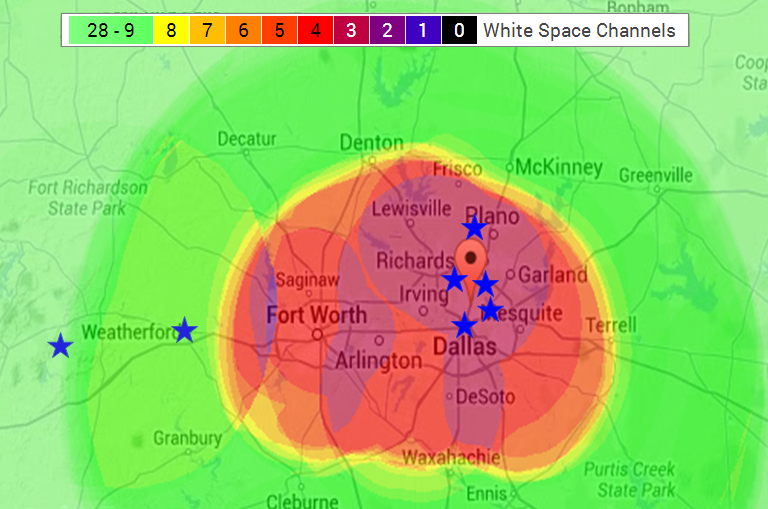
\includegraphics[width=74mm]{figures/drivemap}
%\vspace{-0.1in}
%\caption{DFW Metropolitan Measurement Location}                                                                 
%\label{fig:drivemap}
%\vspace{-0.1in}
%\end{figure}
%   
%\begin{figure}
%%\vspace{-0.0in}
%\centering
%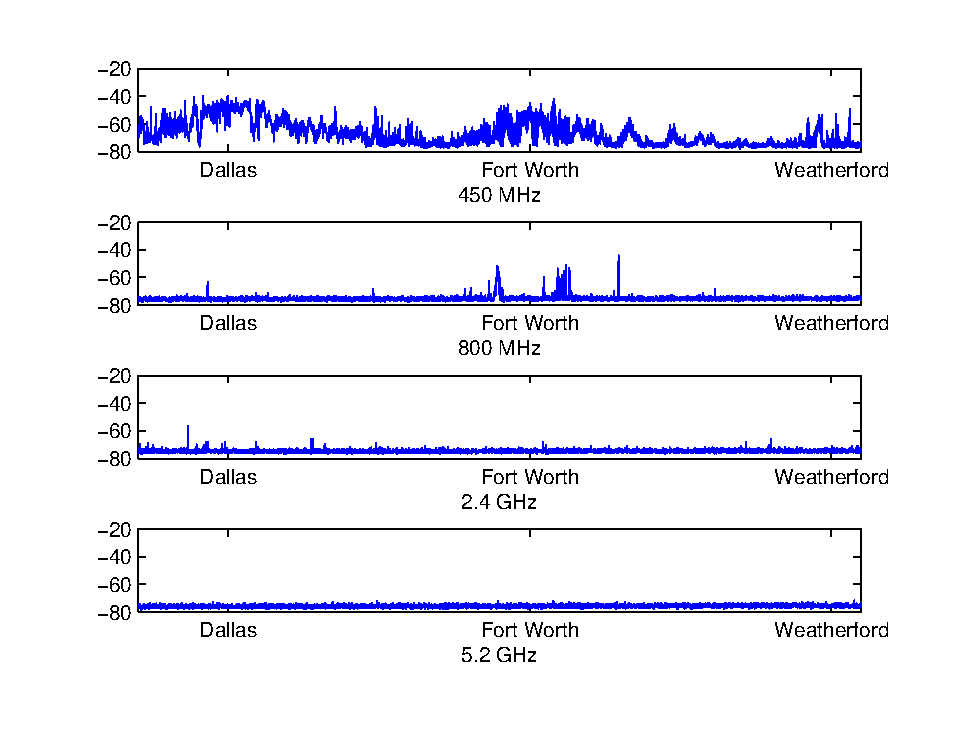
\includegraphics[width=94mm]{figures/drivetest}
%\vspace{-0.1in}
%\caption{Spectrum Activity In DFW}                                                                 
%\label{fig:drivetest}
%\vspace{-0.1in}
%\end{figure}
%
%% Fix location example claiming the activity is kind of stable
%Figure~\ref{fig:labact} depicts an example spectrum utility in activity level
%defined in~\ref{subsec:problem} in our urban lab with the platform introduced 
%in~\ref{sec:experimentdesign}. 
%The activity level from data collected in the same location shows 
%the difference in time domain. On average, the existing signals occupy 25.83 
%percentage of time in 450 MHz, 26.49 percentage of time in 800 MHz, 
%34.95 percentage of time in 2.4 GHz and 35.46 percentage of time in 5.2 GHz. 
%Our experiments show that in a fixed location, the spectrum utility is around
%a certain number in time domain. This character provides a method to tell
%the spectrum utility through measurements. These Inter-network interference 
%of existing signals have to be counted in wireless network deployment. 
%
%   \begin{figure}
%   %\vspace{-0.0in}
%   \centering
%   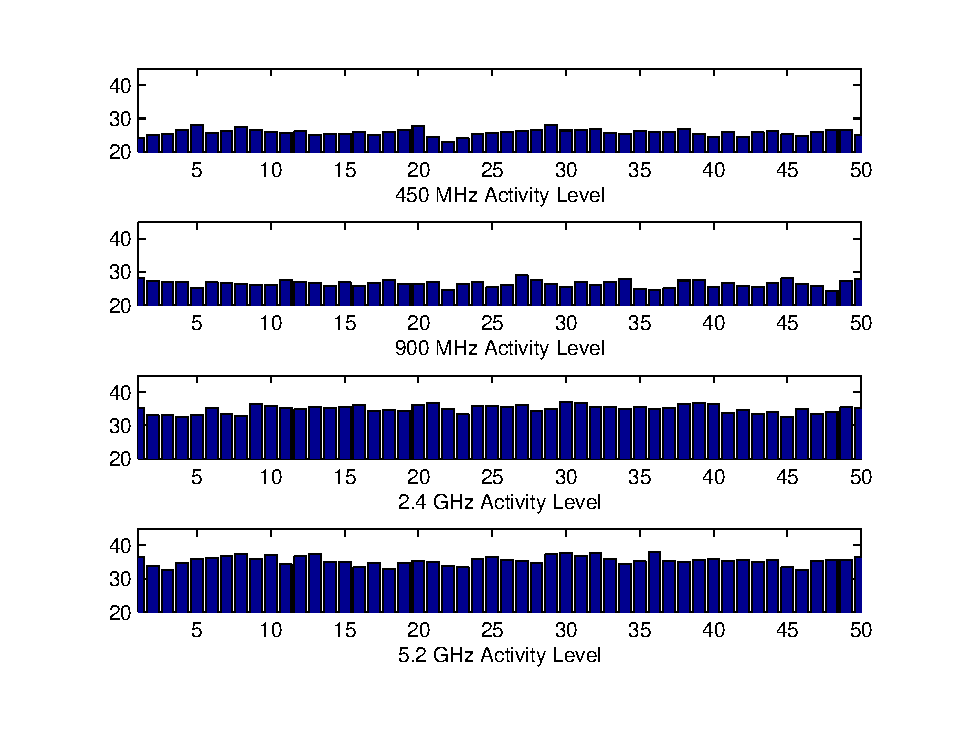
\includegraphics[width=94mm]{figures/labactivity}
%   \vspace{-0.1in}
%   \caption{Wireless Activity in Urban Lab}                                                                 
%   \label{fig:labact}
%   \vspace{-0.1in}
%   \end{figure}
%   
%In the measurements, there is around $10\%$ difference from white space 
%band to WiFi bands in our urban lab. This spectrum utility gap and multiband
%propagation variation in band selection of wireless network 
%deployment is what we have to notice. 
%

\subsection{Model and Problem Formulation}
\label{subsec:problem}

% Assumptions of the network
As opposed to previous works such as~\cite{tang2005interference,yuan2006cross
,si2010overview}, this paper focuses on reducing the inter-network
interference for various population densities for wireless access networks which
jointly employ WiFi and white space bands. We propose a measurement-driven 
framework to estimate the number of access points required for serving the traffic
demand of a certain area. We assume an access point has a limited number of radios
which operate on any channel of a fixed number of channels with the same antenna gain.
Each radio on an access point operates with a classic protocol model~\cite{gupta2000capacity}. 
We further assume that there is a given take rate and traffic demand for a given 
population (as specified in Section~\ref{sec:experimentdesign}).  
%Generally, Internet data request comes with population and Finland government even announce 
%broadband is an individual 'legal right'~\cite{bbcfinland,rosston2011household}. 
%Providing a community wireless Internet service have to satisfy its traffic demand 
%of the people in the area. 
%In populated urban areas, more people need more 
%network capacity in which case WiFi band spatial reuse is better than white space bands
%who limit the capacity in a large area. Moreover, in populated urban area, 
%more Inter-network interference comes from TV station and other sources in white space
%bands could reduce the capacity of a channel. However, in rural area, too many access points
%in WiFi bands for the large area is a waste of funding. Here we are trying to answer the question
% in a certain Inter-network interference, what is the band or bands combination we should 
% use to provide network service for a community with different population density.
%Since mathematical formula is difficult to describe the activities of 
%signal on the air even in an arbitrary area.

For spectrum utility and resulting channel availability, we use a long-term measurement 
for each band.  We define the percentage of sensing samples $S_\theta$ above an 
interference threshold $\theta$ over the total samples $S$ in a time unit as the 
activity level $A$ of inter-network interference:
\begin{equation}
\label{eq:actdef}
A=\frac{S_\theta}{S_a}
\end{equation}
The capacity of a clean channel is denoted by $C$. With the protocol model, the capacity 
of a channel with inter-network interference $C_r$ could be represented as 
the remaining time of the clean channel capacity according to: 
\begin{equation}
\label{eq:intercap}
C_r=C*(1-\bar{A})
\end{equation}

A network deployment should ideally provide network capacity equal to the demand of the service 
area to maintain the capacity constraint. The demand of a service area could be calculated as the 
summation of individual demands all over the service area $D_a=\sum_{p\in P}D_p$. Since 
household demand for Internet has been previously characterized~\cite{rosston2011household}, 
$D_a$ could represent the population distribution $f$ and service area $k$ as 
$D_a=\sum_{f \in F,k \in K}\bar{D_p}*f*k$. 
The capacity constraint could be represented with access points set $M$ according to:
\begin{equation}
\label{eq:nlbound}
\sum_{m \in M}C_r^m \ge \sum_{f \in F,k \in K}\bar{D_p}*f*k
\end{equation}
At the same time, the wireless network must additionally satisfy the coverage constraint in the service 
area where the access points provide connectivity for client devices. 
Generally, a coverage of $95\%$ is acceptable for wireless access networks~\cite{robinson2010deploying}.

In a joint white space and WiFi scenario, the activity level varies according to various interfering 
sources and the propagation characteristics induced by the environmental characteristics of the service area.
A simple method with the least number of access point to cover an area is to use 
multiple orthogonal lower-frequency channels. However, the FCC limits the white space band availability 
for data communication in most metropolitan areas in the United States~\cite{googledatabase}. Moreover, the 
number of channels in each band is limited. Too many lower-frequency channels will cause high levels of 
intra-network interference for the network, which is out of our scope in this work. We assume that the 
cost of the network is proportional to the number of access points required for a given user demand (i.e., due
to the cost of hardware and installation). Therefore, given a geographical region for a new network deployment
we build a measurement-driven framework called Multiband Access Point Estimation (MAPE) to compute the required
number of access points.

\begin{algorithm}[t]
\small
\caption{Multiband Access Point Estimation (MAPE)}
\label{algorithm:mape}
\begin{algorithmic}[1]
\REQUIRE  ~~\\
$A$: Measured Activity Level \\
$F$: Population Distribution\\
$C$: Clean Channel Capacity\\
$n$: Path Loss Exponent \\
$B$: Available frequency bands\\
$M$: Area need to be covered
\STATE Split $M$ in to different type, calculate the traffic demand density $f$
\STATE Calculate in-field channel capacity $C_r$ as $C(1-A)$
\STATE Get the propagation coverage area radius $R_p$ from Frii model based on $n,B,F$
\STATE Calculate the QoS coverage radius $R_{QoS}$ of a Multiband Access Point satisfy the demands of the area
\STATE The coverage radius of a Multiband Access Point is $Min{R_p,R_{QoS}}$
\STATE Apply regular hexagon deployment to get the number of access point for serving given area $M$
\ENSURE ~~\\
The number of Access Points\\
\end{algorithmic}
\end{algorithm}

% Fix the framework , Mark should use them in a single tower with more radios
% Framework
In the space domain, the advantage of higher-frequency channels is the spatial reuse, while
the lower-frequency channels provide greater levels of coverage. Generally, higher 
frequencies are more appropriate for populated areas, and lower frequencies are
more appropriate for sparse areas. The time-domain variation of spectrum utilization 
differs across bands.
%could be seen in Figure~\ref{fig:labact}.
For an internet service provider, the service quality which maps to the capacity constraint must be satisfied.
Given a metropolitan area, the population distribution can be found according to
government statistics~\cite{uscensus}. Then, we can estimate the capacity demand
of each type of area with the assumption that users will exhibit average demand.
According to the population distribution, we split the area into different types,
which compose the space-domain input. Then, we use the measured activity level as 
the time-domain input. We have an average channel capacity of each band according to the 
activity level. With the received signal strength threshold, the Quality-of-Service-constrained
coverage area of different types per channel, and the spatial reuse distance be directly
computed. Then, the maximum area an access point could cover can be calculated as the minimal
area of the QoS-based coverage area and propagation coverage.
Then, the transmit power is adjusted to fulfill the coverage restriction subject to
the FCC regulations for maximum-allowable transmit power. 
A classic regular hexagon deployment process is employed to place the access points.

%With this framework, we combine our measurements to evaluate white
%space bands application varying with population density in section~\ref{sec:experimentdesign}.




%\section{Experiment and Analysis}
\label{sec:experimentdesign}

To study spectrum utility in multiple area types, we developed experiments 
on off-the-shelf wireless platform and remote controlled spectrum analyzer measurement platform.
We do measurement in typical areas of DFW metropolitan carrying these platform.
According to the measured data, we apply our Multiband Access Points Estimation framework to analyze
the performance of white space band application in typical populated areas.

\subsection{Experiment Design}
% Platform
To ensure the results are applicable, we employ a Linux-based 802.11 testbed~\cite{Gateworks}.
The platform includes a Gateworks 2358 board with Ubiquiti XR radios (XR9 at 900 MHz, 
XR2 at 2.4 GHz, XR5 at 5.2 GHz) and a DoodleLabs DL475 radio at 450 MHz~\cite{Ubnt,Gateworks}.
We developed shell script with tcpdump for this testbed working as a sniffer recording all 
802.11 packets.
The experiments taken in downtown Dallas, SMU campus, neighborhood show there is no 802.11
packets dected in white space bands. And in DFW area, as far as we know, we are the only 
group holds FCC license of white space bands. Our experiments verify that these bands 
have not been used for wireless data communication.
However, we observed that Gateworks platform only update its received signal strength when received
a new packet. It is not good for inter-network interference measurement. To cover the gap, 
we employ a spectrum analyzer, multiband antenna, mobile antenna and a laptop developing a spectrum sensing 
system. There is no mobile multiband antenna in market. We compare the multiband antenna measurement
and mobile antenna measurement across bands in lab with our controlled signal source.
Then normalize the received signal strength for mobile antenna measurement.

Our experiment platforms are shown in Figure~\ref{fig:equipment}.
  \begin{figure}
  %\vspace{-0.0in}
  \centering
  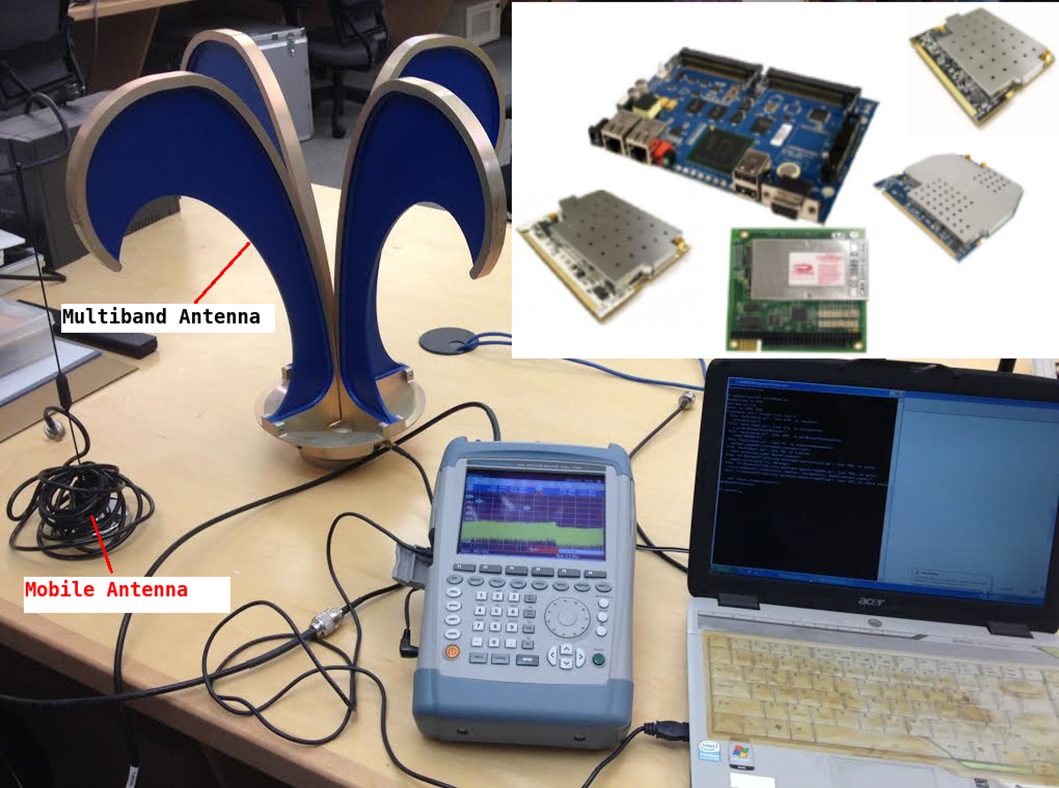
\includegraphics[width=74mm]{figures/equipment}
  \vspace{-0.1in}
  \caption{Multiband Measurement Platform}                                                                 
  \label{fig:equipment}
  %\vspace{-0.0in}
  \end{figure}
We has 32 samples each second from the spectrum analyzer system with time stamp of all bands.
Gateworks sniffer platform record all the packet received with time stamp. The duplicated 
samples are unique through the time stamp. Then we use the uniformed data for activity level
 calculation.  

% Location and Process 
%We apply drive test carrying our platform from Dallas to Weatherford as shown in~\ref{sec:problemformulation}.
We choose typical location according to population distribution and free white space bands 
from Google spectrum database~\cite{googledatabase}. The location chosen for experiments 
are Dallas, Weatherford and Millsap marked with stars in Figure~\ref{fig:drivemap}.
In Weatherford and Millsap, we monitor wireless activities in 3 location for 45 minutes in 
static on a normal weekday. The three locations of a city include downtown, neighborhood and 
rural area. In Dallas, we have multiple measurement in neighborhood, campus and sparse density area.
Then we post-process these data to get the activities level for each band in all the location.
Moreover, through our framework, the number for covering an arbitrary area is calculated and discussed in~\ref{subsec:result}.



\subsection{Results and Analysis} 
\label{subsec:result}

In table~\ref{tab:activitymeasurement}, we show our measurement results in multiple locations of DFW metro.
Dallas as the central city of North Texas, has the highest activities in most of the measured bands,
 especially in 450 MHz. The measurements of Dallas urban are taken from SMU campus, 2 neighborhoods
 and city Plano. We average these data finding 2.4 GHz is more active in urban area rather than 
 downtown area. Most of schools campus and neighborhoods are covered by public or private WiFi today,
which bring more activities in 2.4 GHz and 5.2 GHz.
In Weatherford, all the bands have less activities than Dallas. And due to the measurement location
we chosen, the rural area we chose on the west of Weatherford where could get more interference from
Fort Worth.
Millsap is a typical sparse city has 500 residents total in north Texas. The activities across all the bands are lower than
Dallas, and Weatherford. For 450 MHz, the activity reduce much faster than other bands in Dallas
and Weatherford. 

\begin{table*}
\centering % centering table 
\begin{tabular}{|l|c|c|c|c|c|c|c|c|c|c|c|} % creating 12 columns 
\hline %\hline % inserting double-line 
Bands     & \multicolumn{3}{c|}{Dallas} & \multicolumn{3}{c|}{Weatherford} & \multicolumn{3}{c|}{Millsap} \\% [0.5ex]
\hline % inserts single-line 
% Entering 1st row 
Area Type & Downtown & Urban & Sparse Area & Downtown &  Urban   & Sparse Area & Downtown & Urban & Sparse Area \\ % [0.5ex]
\hline % inserts single-line 
450 MHz &24.3667	&25.8274  &23.7667	&6.050 &12.50  &14.0333 & 7.0000 & 0.0667 & 0.0215 \\      
\hline % inserts single-line                                                                                                       
800 MHz &4.4000 	&16.4940  &4.7667	&5.2167&5.0667 &4.4333  & 3.8667 & 4.2000 & 3.6000 \\      
\hline % inserts single-line                                                                                                      
2.4 GHz &15.8667 	&34.9488  &2.6000	&2.0333&2.0333 &2.7667  & 2.0667 & 1.6000 & 0.8000 \\      
\hline % inserts single-line                                                                                                     
5.2 GHz &19.7000	&35.4571  &1.5333	&1.9333&1.9333 &1.3333  & 1.2667 & 2.0667 & 2.1000 \\      
\hline % inserts single-line 
\end{tabular}    
\label{tab:activitymeasurement}    
\caption{Activity Level in Multiple Locations} % title name of the table 
\vspace{-0.4in}
\end{table*}    

We put these measured activity level into our framework presented in~\ref{algorithm:mape}. We use Millsap
sparse area, Millsap downtown, Weatherford urban, Dallas rural and look up the population density on-line.
We input these information to our framework and calculate the number of access point for covering 
a $13 km \times 13 km$ area in different types. The output is shown in Figure~\ref{fig:redensity}. 

   \begin{figure}
   %\vspace{-0.0in}
   \centering
   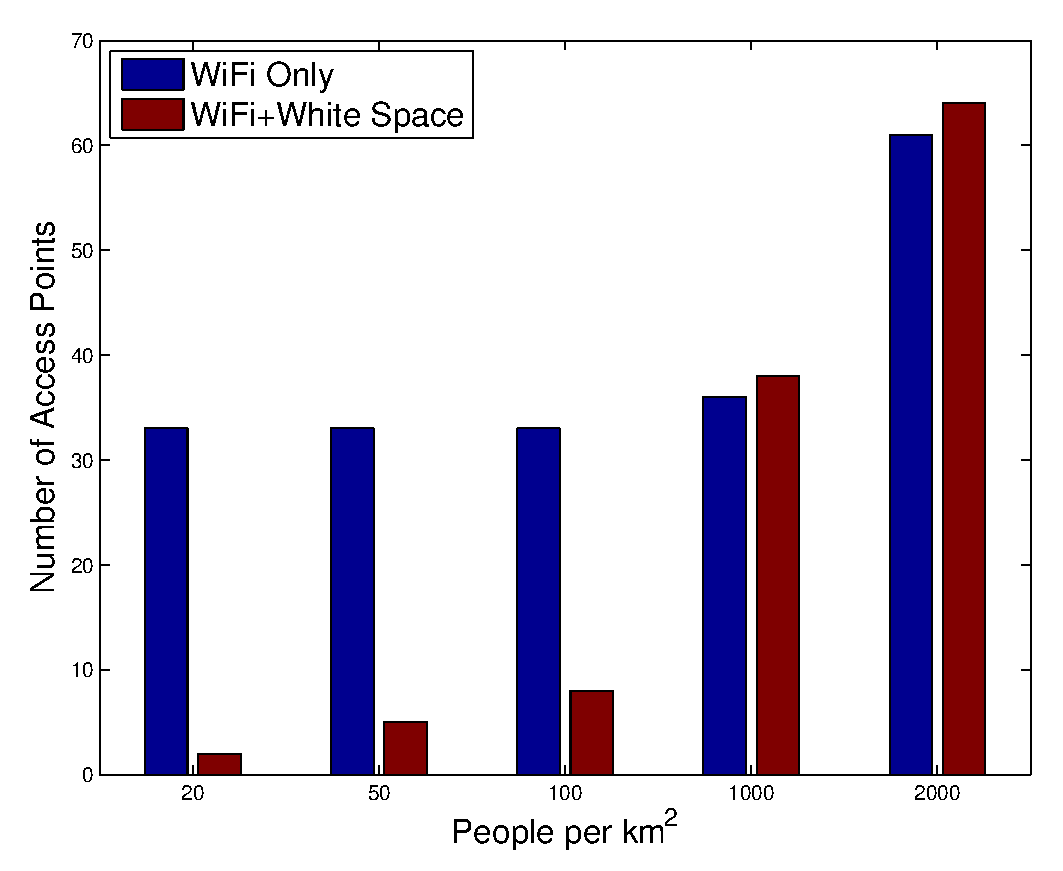
\includegraphics[width=74mm]{figures/redensity}
   \vspace{-0.1in}
   \caption{Number of Access Points need for 13x13 $km^2$ Area}                                                                 
   \label{fig:redensity}
   %\vspace{-0.0in}
   \end{figure}

% Experiment Results & expect results
We set the demand request as $2Mbps$ per person, the population
density as $20,50,100,1000,2000$ per square kilometers. We assume $30\%$ residents will use this
service. For WiFi only, we use 6 channels in 2.4 GHz, and 3 channels in 5.2 GHz. 
We adopt 802.11n maximum data rate 600 Mbps. For WiFi+ White Space
scenario, we use 3 channels in 450 MHz, 2.4 GHz and 5.2 GHz each. Then all the scenarios have the 
same channels in total. As shown in Figure~\ref{fig:redensity},
with the same number of channels, WiFi+White Space gains $1650\%$ comparing to WiFi only in 20 people 
per square kilometer scenario, and $660\%$ in 50 people per square kilometer and $412.5\%$ in 100 people
per square kilometer. But as the population density increase, due to the capacity constraint servicing
people in this area, low frequency white space band lose their advantage of larger communication range. 
And at the same time, the activities of other signal source, such as TV station in downtown area reduce
the capacity of white space band, then WiFi+White Space bands perform worse than WiFi only bands combination.
Moreover, if we count the intra-network interference, the situation could be even worse.


To find the best bands combination, we select 500 people per square kilometer scenario and use Weatherford 
downtown spectrum to calculate the number of access points in this area. We assume the total number of channels 
is 12. The other setup of the experiment is 
the same as the previous configuration. The results are shown in~\ref{fig:varybandcomb}.
   \begin{figure}
   %\vspace{-0.0in}
   \centering
   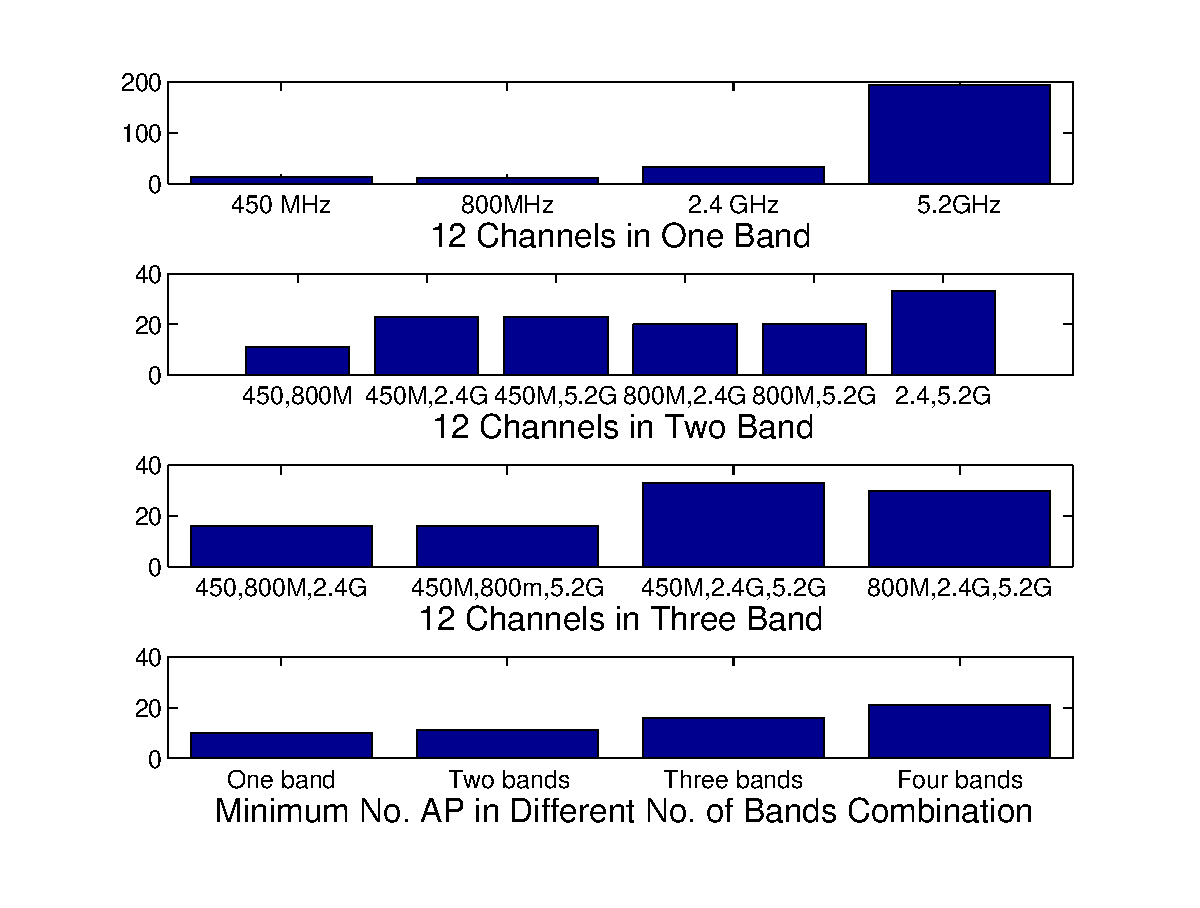
\includegraphics[width=74mm]{figures/varybandcomb}
   \vspace{-0.1in}
   \caption{Bands Combinations of The Same No. of Channels in 500 Population Density}                                                                 
   \label{fig:varybandcomb}
   %\vspace{-0.0in}
   \end{figure}

The first subplot in the Figure is the number of access points needs for 12 channels in one band.
As frequency goes up, more access points need to serve this area. 450 MHz does not outperform 
800 MHz since in this population density, they have the same service area.
Subplot 2 shows if we have equal channels in 2 bands, white space bands combination performs better
than WiFi by 63.64\% and WiFi + white space bands by 56.52\%. In this scenario, the more white space bands channels are 
used, the better performance will be got.

   \begin{figure}
   %\vspace{-0.0in}
   \centering
   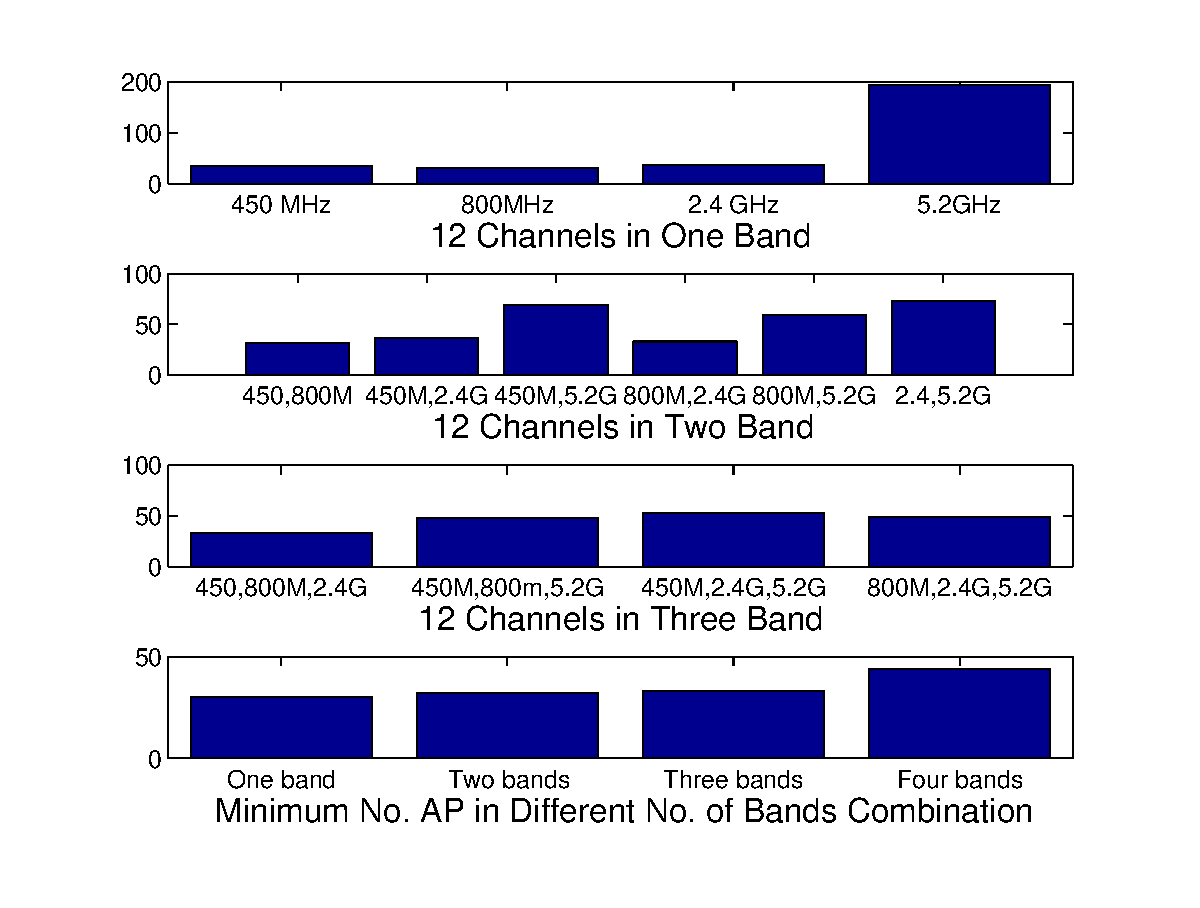
\includegraphics[width=74mm]{figures/varybandcomb2}
   \vspace{-0.1in}
   \caption{Bands Combinations of The Same No. of Channels in 1500 Population} 
   \label{fig:varybandcomb2}
   %\vspace{-0.0in}
   \end{figure}

We reset the population as 1500. And Dallas urban spectrum activity is used in\ref{fig:varybandcomb2}.
In this scenario, using all channels in white space band has the same performance comparing to WiFi+
White space bands. And generally white space band still have benefit reducing the number of access points
by 23.33\% and 9.19\%. As population density increase, the gain brought by white space decrease. The best
band combination is still the combination with white space bands. 


%\section{Related Work}
\label{sec:related}

% White Space large propagation range
With new FCC regulations on the use of white space bands, there are two factors to
consider with such bands: large propagation range and existing inter-network interference from 
TV stations and other devices such as microphones~\cite{fccwhitespace,cui2013leveraging,bahl2009white}.
Prior work does not specifically study the benefits of jointly using white space and WiFi bands in
deployment of wireless access networks~\cite{akyildiz2005wireless}. Additionally, prior work related
to white spaces target opportunistic media access. However, the application of white spaces 
across diverse population densities has not been fully explored.
%outdoor environment, such as urban and rural areas, has not been exploited. Lacking the 
%discussion of white space in outdoor environment is blocking the development of white space
%applications.
 
 % Network propagation difference
Finally, some works discuss the propagation variation in both WiFi bands and white space bands.
For example, Robinson et al. models the propagation variation at the same band in terrain 
domain~\cite{robinson2010deploying}. Another work proposes a databased-driven framework for
designing a white space network with database of primary user (TV station) locations and channel 
occupation~\cite{murty2012senseless}. However, these works do not jointly study
the influence of white space and WiFi bands on network deployment according to their resulting 
propagation variation and spectrum utilization.
%of the space domain and spectrum utility in time domain.

% New Problem: more radios on access points or more access points

%\section{Conclusion}
\label{sec:conclusion}
%In future work, we will adapt our algorithms to be used with dynamically-changing
%network conditions, in the field on large-scale WhiteMesh networks.

%investigated the channel assignment in multi-band scenario to leverage the propagation incluence for mesh network applications. 
%We have presented the multi-band mesh network architecture, a new defination of path interference over network, and analyze the advantages and disadvantages of white space bands.
%According to the analysis, we formally propose Best Path Selection and Growing Spanning Tree algorithms for channel assignment in multi-band network. Simulation results show that our scheme outperforms the existing scheme substantially.
%Dynamic and distributed algorithms for multi-band channel assignment problems will be of our future work.




\bibliographystyle{IEEEtran}

\bibliography{beamforming_coverage}

\end{document}
%This is never printed
